
\section{Results}

\begin{frame}{Results}
  
  Revisiting the model
  $$\begin{cases}
    \begin{array}{rl}
      dM\hspace{-.8em}&=[aMC - \frac{gM(t-\tau)}{1-C(t-\tau)} + \gamma M (1-M-C)]dt+\beta M(1-M)dW,\\
      dC\hspace{-.8em}&=[rC(1-M-C) - dC - aMC]dt.\\
    \end{array}
    \end{cases}$$\\
  We are interested in the effects of:
  \begin{itemize}
  \item $\theta$ (the initial condition)\\
  \item $\beta$\\
  \item $\tau$\\
  \item $g$\\
  \end{itemize}
  
  

\end{frame}

\begin{frame}{Theta}
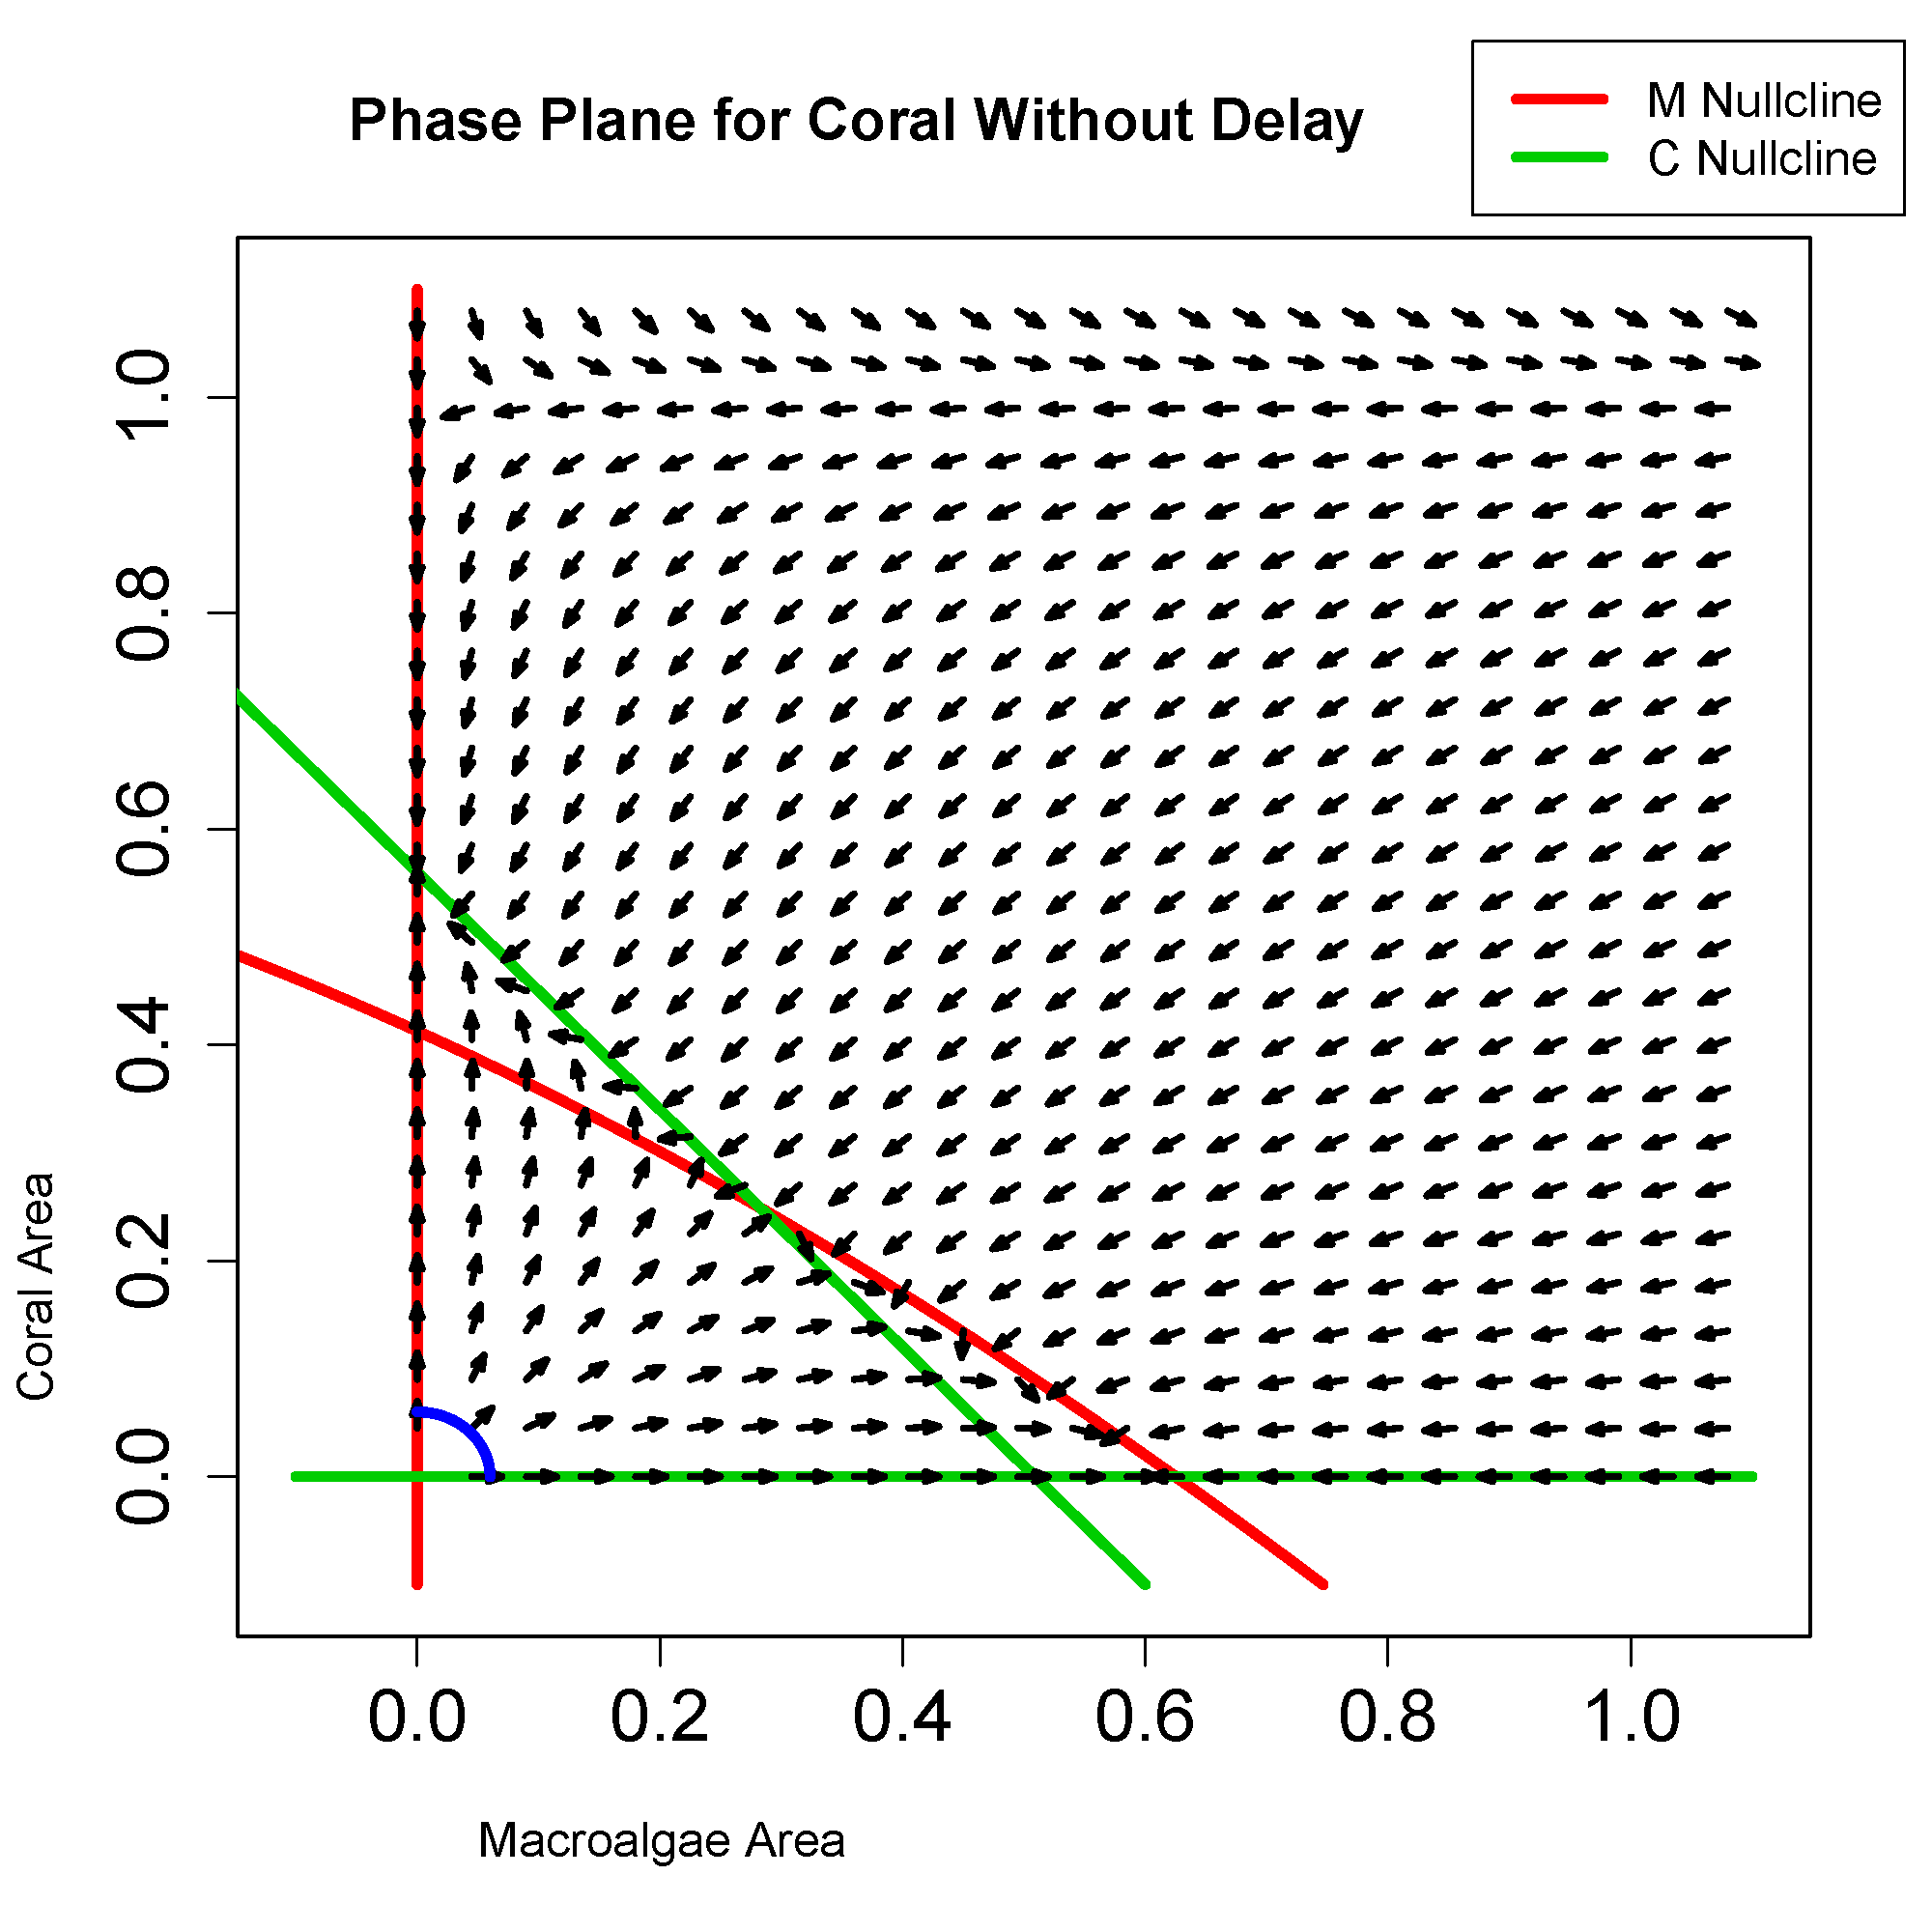
\includegraphics[scale=.325]{./nullclinesarc.pdf}

\end{frame}

\begin{frame}{The Simulation}
We sampled the following values:
\begin{itemize}
\item $\theta$ = $\frac{\pi}{80}$ to $\frac{39\pi}{80}$ by $\frac{\pi}{80}$\\
\item $\beta$ = 0 to 1 by 0.05\\
\item $\tau$ = 0.5 to 1 by 0.05\\
\item $g$ = 0.2 to 0.8 by 0.1\\
\end{itemize}
\end{frame}

\begin{frame}{Initial Conditions}
\includegraphics[scale=.325]{./theta_ic.pdf}
\end{frame}

\begin{frame}{The Three Models}
Based on the plot, we will try the following three models
\begin{itemize}
\item Binomial Logit\\
Fits the model $logit(p)=a+b\theta$ where $logit(p)=log(\frac{p}{1-p})$\\
\item Poisson Log\\
Fits the model $log(y)=a+b\theta$\\
\item Ordinary Least Squares (OLS)\\
Fits the model $p=a+b\theta$\\
\end{itemize}
\end{frame}


\begin{frame}{Binomial Logit, Poisson Log, or OLS}
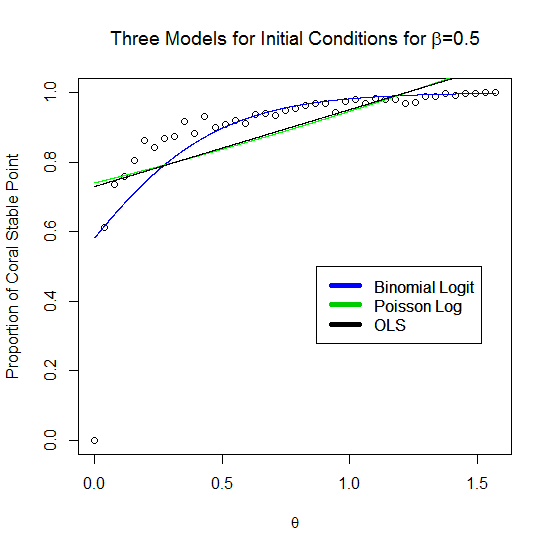
\includegraphics[scale=.425]{theta_three_models.png}
\end{frame}

\begin{frame}\frametitle{The Binomial Logit Model}
{\fontsize{8}{3} \color{blue} \verbatiminput{theta_logit_summary.txt}}

Conducting a goodness of fit test: \\
$P(\chi^{2}_{1}>3288.10-927.62)<0.0001$\\

\end{frame}


%%% Local Variables:
%%% mode: latex
%%% TeX-master: "Presentation2"
%%% End:
